\documentclass{article}
\usepackage{amssymb}
\usepackage{nth}
\usepackage[utf8]{inputenc}
\usepackage{graphicx}
\usepackage[final]{pdfpages}


\title{Number Theory}
\author{Cecilia}
\date{June 2021}

\begin{document}

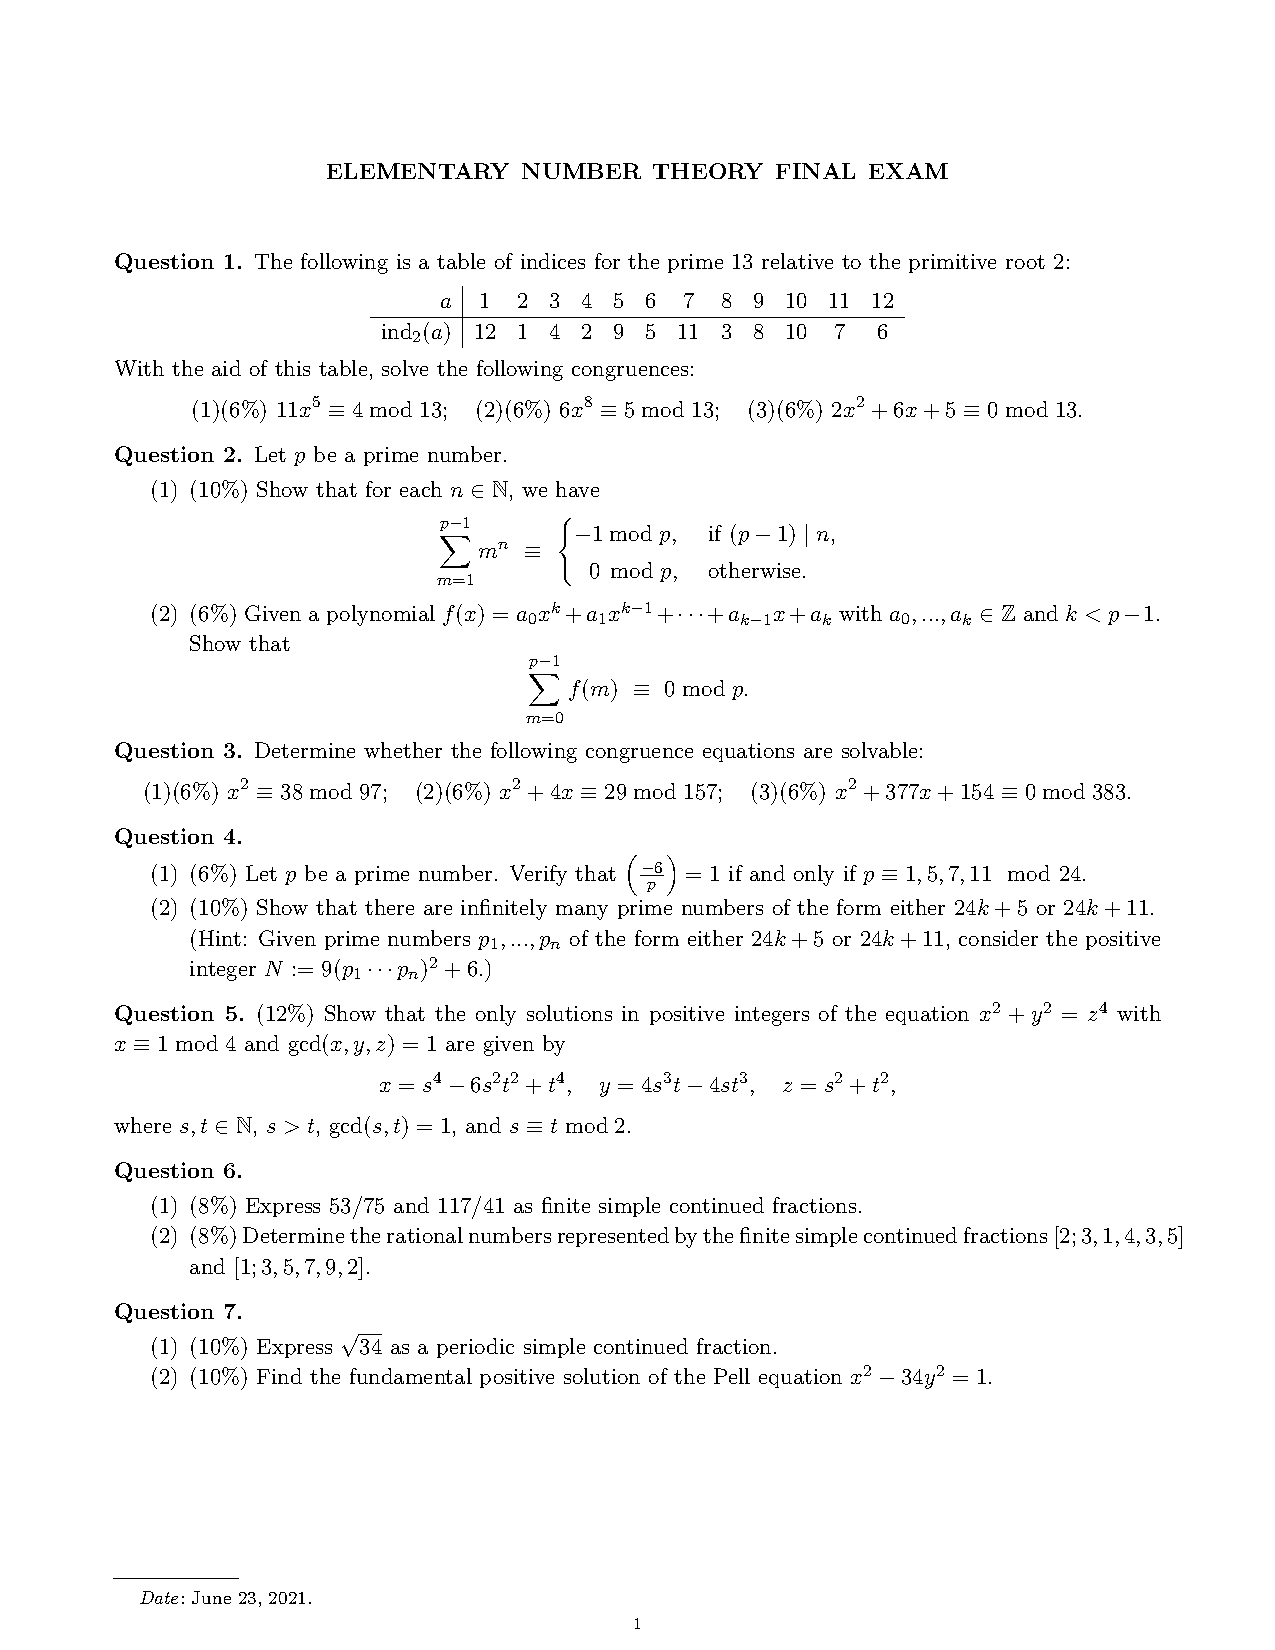
\includepdf[pages=-]{Exams/NumberTheory/Problems/Elementary_Number_Theory_Final_Exam__2021_Spring_.pdf}

\maketitle
\section*{Question 1}
\subsection*{(1)}
\begin{eqnarray*}
        11x^5 & \equiv & 4   \pmod{13} \\
  2^7 (2^y)^5 & \equiv & 2^2 \pmod{13} \\
       7 + 5y & \equiv & 2   \pmod{12} \\
            y & \equiv & 11  \pmod{12} \\
            x & \equiv & 7   \pmod{13}
\end{eqnarray*}
\begin{verbatim}
>> (11 * 7 ** 5) % 13
4
\end{verbatim}

\subsection*{(2)}
\begin{eqnarray*}
         6x^8 & \equiv & 5   \pmod{13} \\
  2^5 (2^y)^8 & \equiv & 2^9 \pmod{13} \\
       5 + 8y & \equiv & 9   \pmod{12} \\
           8y & \equiv & 4   \pmod{12} \\
            y & \equiv & 2   \pmod{12} \\
            x & \equiv & 4   \pmod{13}
\end{eqnarray*}
\begin{verbatim}
>>> (6 * 4 ** 8) % 13
5
\end{verbatim}

\subsection*{(3)}
We observe that $ x \equiv 1 \pmod{13} $ is an obvious answer. By long division (in modular arithmetic of course) we get $ 2x^2 + 6x + 5 = (x - 1)(2x + 8) $. That gives the another solution to be $ x \equiv 9 \pmod{13} $.
\begin{verbatim}
>>> (2 * (1 ** 2) + 6 * 1 + 5) % 13
0
>>> (2 * (9 ** 2) + 6 * 9 + 5) % 13
0
\end{verbatim}

\section*{Question 2}
\subsection*{(1)}
We can represent the number $ 1 \le m < p $ as elements of $ Z_p $. Since $ Z_p $ is cyclic, we can represent them as distinct power of a primitive root $ r $.

\begin{eqnarray*}
  &      & S                                         \\
  &\equiv& \sum\limits_{i = 1}^{p-1}m^n     \pmod{p} \\
  &\equiv& \sum\limits_{i = 1}^{p-1}(r^i)^n \pmod{p} \\
  &\equiv& \sum\limits_{i = 1}^{p-1}(r^n)^i
\end{eqnarray*}

When $ p - 1 | n $, we have $ r^n \equiv 1 \pmod{p} $ by Fermat's theorem. Therefore $ S \equiv p - 1 \equiv -1 \pmod{p} $. Otherwise

\begin{eqnarray*}
  & & S                                              \\
  &\equiv& \sum\limits_{i = 1}^{p-1}(r^n)^i \pmod{p} \\
  &\equiv& \frac{(r^n)^p - r^n}{r^n - 1}    \pmod{p} \\
  &\equiv& \frac{r^n - r^n}{r^n - 1}        \pmod{p} \\
  &\equiv& 0                                \pmod{p} 
\end{eqnarray*}
The \nth{3} equivalence is a consequence of Fermat's theorem.
\subsection*{(2)}
\begin{eqnarray*}
  &      & \sum\limits_{m = 1}^{p-1}f(m) \\
  &\equiv& \sum\limits_{m = 1}^{p-1}\sum\limits_{i = 0}^{k}a_{k-i} m^i \pmod{p} \\
  &\equiv& \sum\limits_{i = 0}^{k}\sum\limits_{m = 1}^{p-1}a_{k-i} m^i \pmod{p} \\
  &\equiv& \sum\limits_{i = 0}^{k}a_{k-i}\sum\limits_{m = 1}^{p-1} m^i \pmod{p} \\
  &\equiv& \sum\limits_{i = 0}^{k}a_{k-i} 0 \pmod{p} \\
  &\equiv& 0
\end{eqnarray*}
The \nth{4} equivalence is a consequence of part 1 as $ k < p - 1 $.

\section*{Question 3}
Manually computing the Legendre's symbol is simply too tedious, the following program is written to leverage quadratic reciprocity to compute Legendre's symbol and have it spill out the \LaTeX code.
\begin{verbatim}
def prime_legendre(a, p):
  if a == 2:
    p8 = p % 8
    if p8 == 1 or p8 == 7:
      answer = 1
    else:
      answer = -1
    print("\\begin{eqnarray*}")
    print("  & & \\left(\\frac{%s}{%s}\\right) \\\\" % (a, p))
    print("  &=& (-1)^{(%s^2 - 1)/8} \\\\" % p)
    print("  &=& %s" % answer)
    print("\\end{eqnarray*}")
    return answer
  else:
    answer = legendre(p % a, a) * (-1)** ((p-1)//2 * (a-1)//2)
    print("\\begin{eqnarray*}")
    print("  & &  \\left(\\frac{%s}{%s}\\right) \\\\" % (a, p))
    print("  &=& \\left(\\frac{%s}{%s}\\right) (-1)^{(\\frac{%s-1}{2}\\frac{%s-1}{2})} \\\\" % (p, a, p, a))
    print("  &=& \\left(\\frac{%s}{%s}\\right) (-1)^{(\\frac{%s-1}{2}\\frac{%s-1}{2})} \\\\" % (p % a, a, p, a))
    print("  &=& %s" % answer)
    print("\\end{eqnarray*}")
    return answer

def legendre(a, p):
  if a == 1:
    return 1
  else:
    s = "  & & \\left(\\frac{%s}{%s}\\right) \\\\\n  &=& " % (a, p)
    terms = []
    answer = 1
    factor = 2
    while a > 1:
      while factor <= a:
        power = 0
        while a % factor == 0:
          a = a // factor
          power = power + 1        
        if power > 0:
          terms.append((factor, power))
          answer = answer * (prime_legendre(factor, p) ** power)
          factor = factor + 1
          break
        else:
          factor = factor + 1
  if len(terms) > 1:
    for (f, power) in terms:
      if power == 1:
        s = s + "\\left(\\frac{%s}{%s}\\right)" % (f, p)
      else:
        s = s + "\\left(\\frac{%s}{%s}\\right)^%s" % (f, p, power)
    s = s + " \\\\\n  &=& %s" % answer
    print("\\begin{eqnarray*}")
    print(s)
    print("\\end{eqnarray*}")
  return answer    
\end{verbatim}
\subsection*{(1)}
\begin{eqnarray*}
  & & \left(\frac{2}{97}\right) \\
  &=& (-1)^{(97^2 - 1)/8} \\
  &=& 1
\end{eqnarray*}
\begin{eqnarray*}
  & & \left(\frac{2}{19}\right) \\
  &=& (-1)^{(19^2 - 1)/8} \\
  &=& -1
\end{eqnarray*}
\begin{eqnarray*}
  & &  \left(\frac{19}{97}\right) \\
  &=& \left(\frac{97}{19}\right) (-1)^{(\frac{97-1}{2}\frac{19-1}{2})} \\
  &=& \left(\frac{2}{19}\right) (-1)^{(\frac{97-1}{2}\frac{19-1}{2})} \\
  &=& -1
\end{eqnarray*}
\begin{eqnarray*}
  & & \left(\frac{38}{97}\right) \\
  &=& \left(\frac{2}{97}\right)\left(\frac{19}{97}\right) \\
  &=& -1
\end{eqnarray*}
Therefore $ x^2 \equiv 38 \pmod{97} $ does not have a solution.
\subsection*{(2)}
\begin{eqnarray*}
  & &  \left(\frac{3}{157}\right) \\
  &=& \left(\frac{157}{3}\right) (-1)^{(\frac{157-1}{2}\frac{3-1}{2})} \\
  &=& \left(\frac{1}{3}\right) (-1)^{(\frac{157-1}{2}\frac{3-1}{2})} \\
  &=& 1
\end{eqnarray*}
\begin{eqnarray*}
  & & \left(\frac{2}{3}\right) \\
  &=& (-1)^{(3^2 - 1)/8} \\
  &=& -1
\end{eqnarray*}
\begin{eqnarray*}
  & &  \left(\frac{3}{11}\right) \\
  &=& \left(\frac{11}{3}\right) (-1)^{(\frac{11-1}{2}\frac{3-1}{2})} \\
  &=& \left(\frac{2}{3}\right) (-1)^{(\frac{11-1}{2}\frac{3-1}{2})} \\
  &=& 1
\end{eqnarray*}
\begin{eqnarray*}
  & &  \left(\frac{11}{157}\right) \\
  &=& \left(\frac{157}{11}\right) (-1)^{(\frac{157-1}{2}\frac{11-1}{2})} \\
  &=& \left(\frac{3}{11}\right) (-1)^{(\frac{157-1}{2}\frac{11-1}{2})} \\
  &=& 1
\end{eqnarray*}
\begin{eqnarray*}
  & & \left(\frac{33}{157}\right) \\
  &=& \left(\frac{3}{157}\right)\left(\frac{11}{157}\right) \\
  &=& 1
\end{eqnarray*}
Therefore $ (x + 2) \equiv 33 \pmod{157} $ has two solutions, and so does $ x^2 + 4x \equiv 29 \pmod{157} $
\begin{verbatim}
>>> (68 * 68 + 4 * 68) % 157
29
>>> (85 * 85 + 4 * 85) % 157
29
\end{verbatim}
\subsection*{(3)}
\begin{eqnarray*}
  & & \left(\frac{2}{383}\right) \\
  &=& (-1)^{(383^2 - 1)/8} \\
  &=& 1
\end{eqnarray*}
\begin{eqnarray*}
  & & \left(\frac{2}{5}\right) \\
  &=& (-1)^{(5^2 - 1)/8} \\
  &=& -1
\end{eqnarray*}
\begin{eqnarray*}
  & &  \left(\frac{5}{7}\right) \\
  &=& \left(\frac{7}{5}\right) (-1)^{(\frac{7-1}{2}\frac{5-1}{2})} \\
  &=& \left(\frac{2}{5}\right) (-1)^{(\frac{7-1}{2}\frac{5-1}{2})} \\
  &=& -1
\end{eqnarray*}
\begin{eqnarray*}
  & &  \left(\frac{7}{383}\right) \\
  &=& \left(\frac{383}{7}\right) (-1)^{(\frac{383-1}{2}\frac{7-1}{2})} \\
  &=& \left(\frac{5}{7}\right) (-1)^{(\frac{383-1}{2}\frac{7-1}{2})} \\
  &=& 1
\end{eqnarray*}
\begin{eqnarray*}
  & & \left(\frac{2}{3}\right) \\
  &=& (-1)^{(3^2 - 1)/8} \\
  &=& -1
\end{eqnarray*}
\begin{eqnarray*}
  & &  \left(\frac{3}{17}\right) \\
  &=& \left(\frac{17}{3}\right) (-1)^{(\frac{17-1}{2}\frac{3-1}{2})} \\
  &=& \left(\frac{2}{3}\right) (-1)^{(\frac{17-1}{2}\frac{3-1}{2})} \\
  &=& -1
\end{eqnarray*}
\begin{eqnarray*}
  & &  \left(\frac{17}{383}\right) \\
  &=& \left(\frac{383}{17}\right) (-1)^{(\frac{383-1}{2}\frac{17-1}{2})} \\
  &=& \left(\frac{9}{17}\right) (-1)^{(\frac{383-1}{2}\frac{17-1}{2})} \\
  &=& 1
\end{eqnarray*}
\begin{eqnarray*}
  & & \left(\frac{238}{383}\right) \\
  &=& \left(\frac{2}{383}\right)\left(\frac{7}{383}\right)\left(\frac{17}{383}\right) \\
  &=& 1
\end{eqnarray*}
Therefore $ (x + 380)^2 \equiv 238 \pmod{383} $ has two solutions, and so does $ x^2 + 377x + 154 \equiv 0 \pmod{383} $. The transformation from $ x^2 + 377x + 154 \equiv 0 \pmod{383} $ to $ (x + 380)^2 \equiv 238 \pmod{383} $ is done simply by completing the square. Notice $ 2^{-1} \pmod{383} = 192 $ so we find $ 380 = 192 \times 377 \pmod{383} $. The rest is obvious.

\begin{verbatim}
>>> (94 ** 2 + 377 * 94 + 154) % 383
0
>>> (295 ** 2 + 377 * 295 + 154) % 383
0
\end{verbatim}

\section*{Question 4}
\subsection*{(1)}
\begin{eqnarray*}
  & & \left(\frac{-6}{p}\right) \\
  &=& \left(\frac{-1}{p}\right)\left(\frac{2}{p}\right)\left(\frac{3}{p}\right) \\
  &=& \left(\frac{-1}{p}\right)\left(\frac{2}{p}\right)\left(\frac{p}{3}\right)(-1)^{\frac{3-1}{2}\frac{p-1}{2}} \\
  &=& A \times B \times C \times D
\end{eqnarray*}
Now we evaluate the values:
\begin{eqnarray*}
  \begin{array}{cccccc}
    p \pmod{24}  &  A &  B &  C &  D & \left(\frac{-6}{p}\right) \\
               1 &  1 &  1 &  1 &  1 &  1 \\
               5 &  1 & -1 & -1 &  1 &  1 \\
               7 & -1 &  1 &  1 & -1 &  1 \\
              11 & -1 & -1 & -1 & -1 &  1 \\
              13 &  1 & -1 &  1 &  1 & -1 \\
              17 &  1 &  1 & -1 &  1 & -1 \\
              19 & -1 & -1 &  1 & -1 & -1 \\
              23 & -1 &  1 & -1 & -1 & -1 \\
  \end{array}
\end{eqnarray*}
So now we verify $ \left(\frac{-6}{p}\right) = 1 \iff p \pmod{12} \in \{1, 5, 7, 11\}$.
\subsection*{(2)}
Qwq

\section*{Question 5}
Since $ x^2 + y^2 = (z^2)^2 $ is a primitive pythagorean triple, we can let $ m > n, (m, n) = 1 $ such that $ x = m^2 - n^2, y = 2mn, z^2 = m^2 + n^2 $. Now we can use the same trick again and let $ s > t, (s, t) = 1 $ such that $ m = s^2 - t^2, n = 2st, z = s^2 + t^2 $. Now we get $ x = m^2 - n^2 = (s^2 - t^2)^2 - (2st)^2 = s^4 - 6s^2t^2 + t^4 $ and $ y = 2mn = 2(s^2 - t^2)2st = 4s^3t - 4st^3 $.

\section*{Question 6}
The repetitive work is best left for the computer, here is the source code for computing finite continued fraction.
\begin{verbatim}
def finite_continued_fraction(n, d):
  result = []
  finite_continued_fraction_helper(n, d, result)
  return result

def finite_continued_fraction_helper(n, d, l):
  if d == 0:
    return
  i = n // d
  l.append(i)
  finite_continued_fraction_helper(d, n - i * d, l)

def expression(continued_fraction_list):
  if len(continued_fraction_list) == 1:
    return str(continued_fraction_list[0])
  else:
    head = continued_fraction_list[0]
    tail = list(continued_fraction_list)
    tail.pop(0)
    return "%s + 1/(%s)" % (head, expression(tail))

def value(continued_fraction_list):
    if len(continued_fraction_list) == 1:
        return (continued_fraction_list[0], 1)
    else:
        head = continued_fraction_list[0]
        tail = list(continued_fraction_list)
        tail.pop(0)
        (n, d) = value(tail)
        return (head * n + d, n)
\end{verbatim}

And here are the results:
\begin{verbatim}
>>> finite_continued_fraction(53, 75)
[0, 1, 2, 2, 2, 4]

>>> finite_continued_fraction(117, 41)
[2, 1, 5, 1, 5]

>>> value([2, 3, 1, 4, 3, 5])
(733, 324)

>>> value([1, 3, 5, 7, 9, 2])
(2911, 2217)
\end{verbatim}

\section*{Question 7}
Again, we will leave the repetitive work to the computer, here is the source code for computing continued fraction and their convergents for an quadratic irrational $ \frac{p + \sqrt{r}}{q} $.
\begin{verbatim}
import math

def quadratic_continued_fraction(p, d, q):
    solution = []
    memo = {}
    start = -1
    while True:
        if (p, q) in memo:
            start = memo[(p, q)]
            break
        alpha = (p + math.sqrt(d))/q
        a = int(alpha)
        memo[(p, q)] = len(solution)
        solution.append(a)
        np = a * q - p
        nq = (d - np * np)//q
        p = np
        q = nq
    return (solution, start)

def convergents(continued_fraction_list):
    p0 = continued_fraction_list[0]
    q0 = 1
    yield (p0, q0)
    q1 = continued_fraction_list[1]
    p1 = p0 * q1 + 1
    yield (p1, q1)
    for i in range(2, len(continued_fraction_list)):
      a = continued_fraction_list[i]
      p2 = a * p1 + p0
      q2 = a * q1 + q0
      yield (p2, q2)
      (p0, p1, q0, q1) = (p1, p2, q1, q2)
\end{verbatim}

And here is the result:
\begin{verbatim}
>>> quadratic_continued_fraction(0, 34, 1)
([5, 1, 4, 1, 10], 1)

>>> for convergent in convergents([5, 1, 4, 1, 10]):
...     print(convergent)
...
(5, 1)
(6, 1)
(29, 5)
(35, 6)
(379, 65)
>>>
\end{verbatim}

That implies the continued fraction representation for $ \sqrt{34} = [5;\overline{1,4,1,10}] $, and the fundamental solution of $ x^2 - 34y^2 = 1 $ is given by $ x = 35 $ and $ y = 6. $. We pick that convergent because the period is 4.

\end{document}
